\documentclass[tikz,border=3mm]{standalone}
\usetikzlibrary{decorations.pathmorphing}
\usepgfmodule{nonlineartransformations}
\makeatletter
\def\nltrafo{%
\pgfmathsetmacro{\myx}{\pgf@x+7*sin(\pgf@x*3.6)}%
\pgf@x=\myx pt}
\makeatother
\begin{document}  
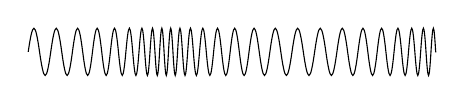
\begin{tikzpicture}
\begin{scope}[transform shape nonlinear=true]
 \pgftransformnonlinear{\nltrafo}
%  \draw[decorate, decoration={coil,aspect=0.3, segment length=2mm, amplitude=3mm}] (0,0) --(10,0);
 \draw[decorate, decoration={coil,aspect=0, segment length=2mm, amplitude=3mm}] (0,-2) --(5,-2);
\end{scope}
\end{tikzpicture}
\end{document}